\documentclass[tikz,border=4pt]{standalone}

\usepackage[T1]{fontenc}
\usepackage[utf8]{inputenc}
\usepackage{tikz}
\usetikzlibrary{positioning, arrows.meta, calc}

\begin{document}

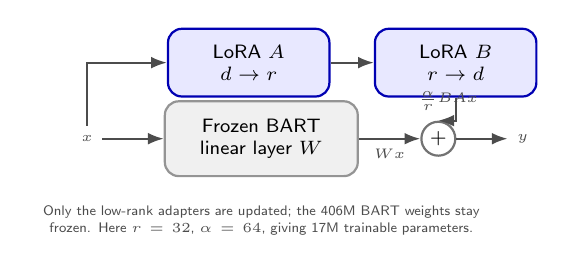
\begin{tikzpicture}[
    every node/.style={font=\sffamily},
    arrow/.style={-{Latex[length=2mm,width=1.5mm]}, thick, draw=black!70},
    train/.style={
        rectangle,
        rounded corners=5pt,
        draw=blue!70!black,
        fill=blue!9,
        thick,
        align=center,
        minimum width=2.05cm,
        minimum height=0.86cm,
        font=\sffamily\scriptsize
    },
    frozen/.style={
        rectangle,
        rounded corners=5pt,
        draw=black!42,
        fill=black!6,
        thick,
        align=center,
        minimum width=2.45cm,
        minimum height=0.95cm,
        font=\sffamily\scriptsize
    },
    sum/.style={
        circle,
        draw=black!55,
        fill=white,
        thick,
        inner sep=1.5pt,
        font=\sffamily\scriptsize
    },
    note/.style={font=\sffamily\tiny, align=center, text=black!70}
]

\node[note] (x) {$x$};
\node[frozen, right=0.78cm of x] (w) {
    Frozen BART\\linear layer $W$
};
\node[train, above right=0.36cm and 0.82cm of x] (a) {
    LoRA $A$\\$d \rightarrow r$
};
\node[train, right=0.55cm of a] (b) {
    LoRA $B$\\$r \rightarrow d$
};
\node[sum, right=0.78cm of w] (plus) {$+$};
\node[note, right=0.65cm of plus] (y) {$y$};

\draw[arrow] (x) -- (w);
\draw[arrow] (w) -- node[below, note] {$Wx$} (plus);
\draw[arrow] (x.north) |- (a.west);
\draw[arrow] (a) -- (b);
\draw[arrow] (b.south) |- node[pos=0.72, above, note] {$\frac{\alpha}{r}BAx$} (plus.north);
\draw[arrow] (plus) -- (y);

\node[note, below=0.24cm of w, text width=5.7cm] {
    Only the low-rank adapters are updated; the 406M BART weights stay frozen.
    Here $r=32$, $\alpha=64$, giving 17M trainable parameters.
};

\end{tikzpicture}

\end{document}
